% !TEX program = xelatex
\documentclass[aspectratio=169, 10pt]{beamer}

\usetheme{Madrid}
\usecolortheme{whale}

% 字体配置
\usepackage{fontspec}
\setmainfont{Times New Roman}
\setsansfont{Arial}
\setmonofont{Consolas}

% 中文支持
\usepackage[UTF8, heading=false]{ctex}

\usepackage{graphicx}
\usepackage{listings}
\usepackage{xcolor}
\usepackage{booktabs}
\usepackage{tikz}
\usetikzlibrary{shapes.geometric, arrows.meta, positioning, calc}
\usepackage{pgfplots}
\pgfplotsset{compat=1.18}
\usepackage{hyperref}
\usepackage{amsmath}

% 代码样式 - 基本设置
\lstset{
  basicstyle=\ttfamily\scriptsize,
  keywordstyle=\color{blue!70}\bfseries,
  commentstyle=\color{gray},
  stringstyle=\color{red!60},
  breaklines=true,
  frame=single,
  rulesepcolor=\color{blue!20!green!20},
  numbers=left,
  numberstyle=\tiny\color{gray},
  tabsize=4,
  showstringspaces=false,
  escapechar=`,
}

% Go 语言关键字
\lstdefinelanguage{Go}{
  morekeywords={func, package, import, return, var, const, for, range, go, chan, defer, if, else, switch, case, default, select, break, continue, struct, interface, type, map, make},
  sensitive=true,
  morecomment=[l]{//},
  morecomment=[s]{/*}{*/},
  morestring=[b]",
}

% Java 语言关键字
\lstdefinelanguage{Java}{
  morekeywords={public, class, static, void, int, long, String, try, var, for, new, return, throws, Exception, import},
  sensitive=true,
  morecomment=[l]{//},
  morecomment=[s]{/*}{*/},
  morestring=[b]",
}

% 标题信息
\title[协程技术调研]{协程技术调研}
\subtitle{从并发演进到底层原理 · 语言对比 · 实验验证}
\author[kyc]{kyc}
\institute{计算机学院}
\date{2026 年 6 月}

\begin{document}

% ==================== 标题页 ====================
\begin{frame}
  \titlepage
\end{frame}

\begin{frame}{核心结论先行}
  \begin{block}{一句话}
    协程不是把 CPU 计算变快的魔法，而是用更低的内存和调度成本处理\textbf{大量等待中的 I/O 任务}。
  \end{block}

  \begin{enumerate}
    \item \textbf{Why}：进程/线程解决并发，但在 C10K/C10M 规模下被栈空间和内核调度成本限制。
    \item \textbf{How}：协程把回调式事件循环包装成可暂停函数，底层依赖编译器状态机、运行时调度器和 OS I/O 多路复用。
    \item \textbf{When}：I/O 密集、高并发、等待多时值得用；CPU 密集仍应依赖多核并行、SIMD 或 GPU。
  \end{enumerate}
\end{frame}

% ==================== 目录 ====================
\begin{frame}{目录}
  \tableofcontents
\end{frame}

% ================================================================
%  第一部分：Why — 为什么需要协程
% ================================================================
\section{为什么需要协程：并发演进}

\begin{frame}{并发模型的演进}
  \begin{center}
  \begin{tikzpicture}[
    node distance=1.2cm,
    box/.style={rectangle, rounded corners, draw=blue!60, fill=blue!8, thick, minimum width=2.4cm, minimum height=0.9cm, align=center, font=\small},
    arr/.style={-{Stealth[length=3mm]}, thick, gray!70},
    note/.style={font=\tiny, text=red!70!black, align=center},
  ]
    \node[box] (A) {多进程\\{\tiny fork/IPC}};
    \node[box, right=of A] (B) {多线程\\{\tiny pthread/锁}};
    \node[box, right=of B] (C) {事件循环\\{\tiny epoll+回调}};
    \node[box, right=of C] (D) {协程\\{\tiny 可暂停的函数}};
    \draw[arr] (A) -- (B);
    \draw[arr] (B) -- (C);
    \draw[arr] (C) -- (D);
    \node[note, below=0.2cm of A] {开销大};
    \node[note, below=0.2cm of B] {$\sim$1MB栈\\内核切换贵};
    \node[note, below=0.2cm of C] {回调地狱\\状态难维护};
    \node[note, below=0.2cm of D, text=green!50!black] {线性代码\\异步执行};
  \end{tikzpicture}
  \end{center}

  \vspace{0.3cm}
  \begin{itemize}
    \item \textbf{线程让步于规模}：C10K $\to$ C10M，线程数撞到内存/调度天花板
    \item \textbf{回调让步于可读性}：epoll + callback 性能好，但代码反人类
    \item \textbf{协程是「鱼与熊掌」的妥协}：\textit{线性的代码 + 异步的执行}
  \end{itemize}
\end{frame}

\begin{frame}{四种并发模型对比}
  \centering
  \small
  \begin{tabular}{lcccccc}
    \toprule
    \textbf{维度} & \textbf{进程} & \textbf{线程} & \textbf{事件循环} & \textbf{协程} \\
    \midrule
    调度方     & OS 抢占 & OS 抢占 & 用户态 & 用户态(协作) \\
    切换开销   & 数十 $\mu$s & 1--5 $\mu$s & $\sim$10 ns & 10--100 ns \\
    栈空间     & MB 级 & $\sim$1 MB & 无(堆闭包) & 2--8 KB \\
    编码风格   & IPC 复杂 & 线性+锁 & 嵌套回调 & 线性+await \\
    典型规模   & 百级 & 千级 & 万--十万 & \textbf{百万级} \\
    适合场景   & 强隔离 & CPU 密集 & 底层网络 & \textbf{I/O 密集} \\
    \bottomrule
  \end{tabular}

  \vspace{0.5cm}
  \begin{block}{一句话总结}
    协程 = 用户态调度的、可暂停-恢复的函数，把「事件循环 + 状态机」从手写变成编译器/运行时生成。
  \end{block}
\end{frame}

% ================================================================
%  第二部分：What — 协程定义与分类
% ================================================================
\section{协程的定义、分类与心智模型}

\begin{frame}[fragile]{协程是什么：把 callback 还原为函数}
  \begin{columns}[T]
    \begin{column}{0.48\textwidth}
      \textbf{协程视角}
      \begin{lstlisting}[language=C++, title={线性、可读}]
Task<Response> handle(Request req) {
  auto user = co_await db.query(uid);
  auto data = co_await rpc.fetch(user);
  co_return render(data);
}
      \end{lstlisting}
    \end{column}
    \begin{column}{0.48\textwidth}
      \textbf{回调视角}
      \begin{lstlisting}[language=Python, title={嵌套、难维护}]
def handle(req, cb):
  db.query(uid, lambda user:
    rpc.fetch(user, lambda data:
      cb(render(data))))
      \end{lstlisting}
    \end{column}
  \end{columns}

  \vspace{0.3cm}
  \begin{alertblock}{关键认知}
    协程不是「更快」，是把\textit{隐式}的状态机变成\textit{显式}由编译器生成。运行时复杂度不变，开发心智复杂度大大降低。
  \end{alertblock}
\end{frame}

\begin{frame}{协程的两个分类维度}
  \begin{columns}[T]
    \begin{column}{0.48\textwidth}
      \textbf{是否有独立栈}\\[0.3cm]
      \textcolor{blue!70}{\textbf{有栈协程 (Stackful)}}
      \begin{itemize}
        \item 每个协程一段独立栈
        \item 切换 = 切寄存器 + SP
        \item 任意深度都能 yield
        \item 代表：\textbf{Go、Lua}
      \end{itemize}
      \vspace{0.2cm}
      \textcolor{orange!80!black}{\textbf{无栈协程 (Stackless)}}
      \begin{itemize}
        \item 编译为状态机
        \item 局部变量存到堆上 frame
        \item 只能在顶层 await
        \item 代表：\textbf{C++20、Python、C\#}
      \end{itemize}
    \end{column}
    \begin{column}{0.48\textwidth}
      \textbf{调度对称性}\\[0.3cm]
      \textcolor{blue!70}{\textbf{对称协程}}
      \begin{itemize}
        \item 协程之间互相 yield
        \item 类似 goroutine
      \end{itemize}
      \vspace{0.2cm}
      \textcolor{orange!80!black}{\textbf{非对称协程}}
      \begin{itemize}
        \item 有明确的 caller/callee
        \item yield 必回到调用者
        \item 类似 generator、async/await
      \end{itemize}

      \vspace{0.4cm}
      \begin{block}{主流趋势}
        非对称 + 无栈 + 调度器驱动\\
        更省内存，更利于编译器优化
      \end{block}
    \end{column}
  \end{columns}
\end{frame}

% ================================================================
%  第三部分：How — 底层机制
% ================================================================
\section{底层机制：有栈 vs 无栈}

\begin{frame}{无栈协程：编译器把函数变成状态机}
  \begin{center}
  \begin{tikzpicture}[
    node distance=0.8cm,
    box/.style={rectangle, rounded corners, draw=blue!50, fill=blue!5, minimum width=3cm, minimum height=0.7cm, align=center, font=\small},
    arr/.style={-{Stealth[length=2.5mm]}, thick, blue!60},
  ]
    \node[box] (src) {源码:\\{\tiny co\_await a; co\_await b;}};
    \node[box, below=of src] (compiler) {编译器重写};
    \node[box, below left=0.8cm and 1cm of compiler] (frame) {堆分配 Frame:\\{\tiny 局部变量+状态号+恢复指针}};
    \node[box, below right=0.8cm and 1cm of compiler] (sm) {switch(state)\\{\tiny case 0: ... suspend}\\{\tiny case 1: ... return}};
    \draw[arr] (src) -- (compiler);
    \draw[arr] (compiler) -- (frame);
    \draw[arr] (compiler) -- (sm);
  \end{tikzpicture}
  \end{center}

  \vspace{0.2cm}
  \begin{columns}[T]
    \begin{column}{0.45\textwidth}
      \begin{exampleblock}{优点}
        \begin{itemize}
          \item 无需独立栈
          \item 单协程内存 $\approx$ 几十--几百字节
          \item 切换 $\approx$ 一次间接跳转
        \end{itemize}
      \end{exampleblock}
    \end{column}
    \begin{column}{0.45\textwidth}
      \begin{alertblock}{缺点}
        \begin{itemize}
          \item 必须由编译器改写
          \item co\_await 不能嵌进任意函数深处
          \item C++20：标准库无调度器/Task/IO
        \end{itemize}
      \end{alertblock}
    \end{column}
  \end{columns}
\end{frame}

\begin{frame}[fragile]{有栈协程：栈切换的约20行汇编}
  \begin{columns}[T]
    \begin{column}{0.55\textwidth}
      \textbf{核心操作}：保存 callee-saved 寄存器 → 切 RSP → 恢复寄存器 → ret
      \begin{lstlisting}[title={x86\_64 协程切换 (简化)}]
switch_ctx:
    push   rbp
    push   rbx
    push   r12-r15       ; callee-saved
    mov    [rdi], rsp    ; save old SP
    mov    rsp, [rsi]    ; switch SP
    pop    r15-r12
    pop    rbx
    pop    rbp
    ret                   ; jump to new
      \end{lstlisting}
    \end{column}
    \begin{column}{0.4\textwidth}
      \small
      \begin{tabular}{lcc}
        \toprule
        & \textbf{有栈} & \textbf{无栈} \\
        \midrule
        切换成本 & 20--100 ns & 5--20 ns \\
        内存 & KB 级 & 字节级 \\
        实现 & 汇编+栈管理 & 编译器改写 \\
        代表 & Go, ucontext & C++20, Rust \\
        \bottomrule
      \end{tabular}
    \end{column}
  \end{columns}
\end{frame}

% ================================================================
%  第四部分：应用范式
% ================================================================
\section{三大应用范式}

\begin{frame}[fragile]{应用范式：async/await · CSP · 结构化并发}
  \begin{columns}[T]
    \begin{column}{0.32\textwidth}
      \textcolor{blue!70}{\textbf{1. async/await}}\\[0.15cm]
      非对称、无栈\\与 Future/Task 协作
      \begin{lstlisting}[language=Python, basicstyle=\ttfamily\tiny]
async def fetch():
    r = await http.get(url)
    return r.json()
      \end{lstlisting}
      {\tiny C++20 / Python / C\# / Rust}
    \end{column}
    \begin{column}{0.32\textwidth}
      \textcolor{orange!80!black}{\textbf{2. CSP / Channel}}\\[0.15cm]
      对称、有栈\\通过 channel 通信
      \begin{lstlisting}[language=Go, basicstyle=\ttfamily\tiny]
ch := make(chan int)
go func() {
    ch <- compute()
}()
v := <-ch
      \end{lstlisting}
      {\tiny Go、Kotlin}
    \end{column}
    \begin{column}{0.32\textwidth}
      \textcolor{green!50!black}{\textbf{3. 结构化并发}}\\[0.15cm]
      父协程持有子协程生命周期
      \begin{lstlisting}[language=Java, basicstyle=\ttfamily\tiny]
coroutineScope {
  val a = async { f1() }
  val b = async { f2() }
  a.await() + b.await()
}
      \end{lstlisting}
      {\tiny Kotlin、Swift、Trio}
    \end{column}
  \end{columns}

  \vspace{0.4cm}
  \begin{block}{选范式 $\approx$ 选「错误传播 + 取消语义」}
    await 走异常，channel 走信号值，结构化并发自动 cancel。
  \end{block}
\end{frame}

% ================================================================
%  第五部分：语言对比
% ================================================================
\section{主流语言协程支持对比}

\begin{frame}{语言支持总览}
  \centering
  \small
  \begin{tabular}{llllll}
    \toprule
    \textbf{语言} & \textbf{关键字} & \textbf{类型} & \textbf{调度器} & \textbf{版本} & \textbf{函数颜色？} \\
    \midrule
    C++20 & co\_await & 无栈/非对称 & 用户自带 & 2020 & 是 \\
    Go & go, chan & \textbf{有栈}/对称 & GMP 内建 & 2012 & \textbf{否} \\
    Python & async/await & 无栈/非对称 & 单线程循环 & 2015 & 是 \\
    C\# & async/await & 无栈/非对称 & 线程池 & 2012 & 是 \\
    Java 21 & Virtual Thread & \textbf{有栈}/对称 & ForkJoin & 2023 & \textbf{否} \\
    Rust & async/await & 无栈/非对称 & 第三方(tokio) & 2019 & 是 \\
    \bottomrule
  \end{tabular}

  \vspace{0.3cm}
  \begin{alertblock}{「函数颜色」问题}
    async 函数和普通函数互不兼容。\textbf{Go 和 Java 21 通过有栈协程把它消除了}——这是两家的核心卖点。
  \end{alertblock}
\end{frame}

\begin{frame}[fragile]{C++20：标准只给「机制」，运行时全靠你}
  \begin{lstlisting}[language=C++, title={C++20 协程最小示例}]
struct Task {
  struct promise_type {
    Task get_return_object() { return {}; }
    std::suspend_never initial_suspend() { return {}; }
    std::suspend_always final_suspend() noexcept { return {}; }
    void return_void() {}
    void unhandled_exception() {}
  };
};
Task demo() {
  std::cout << "hello ";
  co_await std::suspend_always{};
  std::cout << "world";
}
  \end{lstlisting}

  \begin{itemize}
    \item 编译器看到 co\_await/co\_yield/co\_return → 函数改写为状态机
    \item 自动生成 frame、resume()、destroy()
    \item \textbf{标准库没有调度器、没有 Task、没有 IO}：需自己写或用 cppcoro/libcoro/asio
  \end{itemize}
\end{frame}

\begin{frame}{Go：GMP 调度器（最成功的有栈协程）}
  \begin{center}
  \begin{tikzpicture}[
    node distance=0.6cm,
    g/.style={circle, draw=green!60, fill=green!10, minimum size=0.5cm, inner sep=1pt, font=\tiny},
    p/.style={rectangle, rounded corners, draw=blue!60, fill=blue!10, minimum width=1.5cm, minimum height=0.6cm, align=center, font=\small},
    m/.style={rectangle, rounded corners, draw=red!60, fill=red!10, minimum width=1.2cm, minimum height=0.5cm, align=center, font=\small},
    arr/.style={-{Stealth[length=2mm]}, thick},
    note/.style={font=\tiny, text=gray},
  ]
    % Local run queue
    \node[g] (g1) at (0,0) {G};
    \node[g, right=0.3cm of g1] (g2) {G};
    \node[g, right=0.3cm of g2] (g3) {G};
    \node[note, below=0.1cm of g1] {本地队列};

    % P
    \node[p, below=0.6cm of g2] (p) {P: 逻辑处理器};
    \draw[arr] (g1.south) -- (p.north west);
    \draw[arr] (g2.south) -- (p.north);
    \draw[arr] (g3.south) -- (p.north east);

    % M
    \node[m, below=0.5cm of p] (m) {M: OS 线程};
    \draw[arr] (p) -- (m);

    % Global run queue
    \node[g, right=2.5cm of g2] (gx) {G};
    \node[note, above=0.1cm of gx] {全局队列};
    \draw[arr, dashed] (gx) -- (p) node[midway, above, font=\tiny] {偷取};

    % CPU
    \node[rectangle, draw=gray, fill=gray!10, minimum width=0.8cm, minimum height=0.5cm, font=\small, below=0.5cm of m] (cpu) {CPU};
    \draw[arr] (m) -- (cpu);

    % Work stealing
    \node[p, right=3cm of p] (p2) {P};
    \draw[arr, dashed, bend left=20] (p.east) to node[above, font=\tiny] {work stealing} (p2.west);
  \end{tikzpicture}
  \end{center}

  \vspace{0.2cm}
  \begin{columns}[T]
    \begin{column}{0.48\textwidth}
      \begin{itemize}
        \item \textbf{G} = goroutine (2KB 起步栈)
        \item \textbf{M} = 内核线程 (GOMAXPROCS)
        \item \textbf{P} = 调度上下文
      \end{itemize}
    \end{column}
    \begin{column}{0.48\textwidth}
      \begin{itemize}
        \item 网络 poller 集成 epoll/kqueue/IOCP
        \item Go 1.14+ 基于信号 SIGURG 的\textbf{抢占式调度}
      \end{itemize}
    \end{column}
  \end{columns}
\end{frame}

\begin{frame}[fragile]{Java 21 虚拟线程：「同步语法 + 协程性能」}
  \begin{lstlisting}[language=Java, title={百万并发虚拟线程}]
try (var exec = Executors.newVirtualThreadPerTaskExecutor()) {
    for (int i = 0; i < 1_000_000; i++)
        exec.submit(() -> { var r = http.send(req); return r; });
}
  \end{lstlisting}

  \begin{itemize}
    \item \textbf{Virtual Thread = JVM 管理的有栈协程}（Continuation + Scheduler）
    \item 跑在少量 carrier 平台线程上，由 ForkJoinPool 调度
    \item JDK 内所有阻塞 API 已改造为 yield 而非 block
    \item \textbf{最大卖点}：旧业务代码一行不改，Thread 换 Thread.ofVirtual() 就能扩到百万并发
  \end{itemize}

  \begin{alertblock}{Pinning 陷阱}
    synchronized 块、JNI 调用会把虚拟线程钉在 carrier 上
  \end{alertblock}
\end{frame}

% ================================================================
%  第六部分：三方协同
% ================================================================
\section{编译器 × 运行时 × 操作系统}

\begin{frame}{三方协同：编译器 · 运行时 · 操作系统}
  \begin{center}
  \begin{tikzpicture}[
    node distance=0.6cm,
    layerblue/.style={rectangle, rounded corners, draw=blue!60, fill=blue!5, minimum width=10cm, minimum height=1.4cm, align=left, font=\small, inner sep=6pt},
    layerorange/.style={rectangle, rounded corners, draw=orange!60, fill=orange!5, minimum width=10cm, minimum height=1.4cm, align=left, font=\small, inner sep=6pt},
    layergreen/.style={rectangle, rounded corners, draw=green!60, fill=green!5, minimum width=10cm, minimum height=1.4cm, align=left, font=\small, inner sep=6pt},
    arrblue/.style={-{Stealth[length=3mm]}, thick, blue!60},
    arrorange/.style={-{Stealth[length=3mm]}, thick, orange!60},
    arrgreen/.style={-{Stealth[length=3mm]}, thick, green!60},
  ]
    \node[layerblue] (compiler) at (0, 3) {
      \textbf{1. 编译器} \hfill 识别 async/await → 重写为状态机 → 分配 frame
    };
    \node[layerorange] (runtime) at (0, 1.2) {
      \textbf{2. 语言运行时} \hfill 调度器(本地队列+work stealing) \quad Task/Future \quad 网络 poller
    };
    \node[layergreen] (os) at (0, -0.6) {
      \textbf{3. 操作系统} \hfill epoll\_wait \quad io\_uring \quad 线程切换
    };
    \draw[arrblue] (compiler) -- (runtime);
    \draw[arrorange] (runtime) -- (os);
    \draw[arrgreen, bend left=30] (os.east) to node[right, font=\tiny] {fd 就绪事件} (runtime.east);
    \draw[arrblue, bend left=30] (runtime.west) to node[left, font=\tiny] {resume} (compiler.west);
  \end{tikzpicture}
  \end{center}

  \vspace{0.3cm}
  \centering
  \small
  \begin{tabular}{lll}
    \toprule
    \textbf{层} & \textbf{干什么} & \textbf{关键点} \\
    \midrule
    编译器 & 把同步代码改写为可暂停 & 状态机 + frame 布局 \\
    运行时 & 调度协程、管理 Task、对接 I/O & work stealing、IO poller \\
    操作系统 & 提供非阻塞 I/O 多路复用 & epoll / kqueue / io\_uring / IOCP \\
    \bottomrule
  \end{tabular}
\end{frame}

% ================================================================
%  第七部分：实验
% ================================================================
\section{实验：协程 vs 多线程}

\begin{frame}{实验设计}
  \textbf{目标}：在相同硬件、相同负载下，对比三种模型的\textbf{吞吐 / 内存 / 切换成本}。

  \vspace{0.3cm}
  \begin{columns}[T]
    \begin{column}{0.48\textwidth}
      \textbf{测试用例}
      \begin{enumerate}
        \item \textbf{I/O 密集}：10000 个并发任务，每个 sleep(0.1s)
        \item \textbf{CPU 密集}：10000 个并发任务，斐波那契(n=25)
        \item \textbf{上下文切换}：百万次 yield/resume
      \end{enumerate}
    \end{column}
    \begin{column}{0.48\textwidth}
      \textbf{对比对象}
      \begin{itemize}
        \item Python：threading vs asyncio
        \item Go：goroutine（GMP 调度器）
        \item Java：平台线程池 vs Virtual Thread
      \end{itemize}
      \vspace{0.2cm}
      \textbf{指标}\\
      吞吐 (req/s)、P99 延迟、RSS 内存、CPU 时间
    \end{column}
  \end{columns}
\end{frame}

\begin{frame}{实验结果：I/O 密集型}
  \centering
  \small

  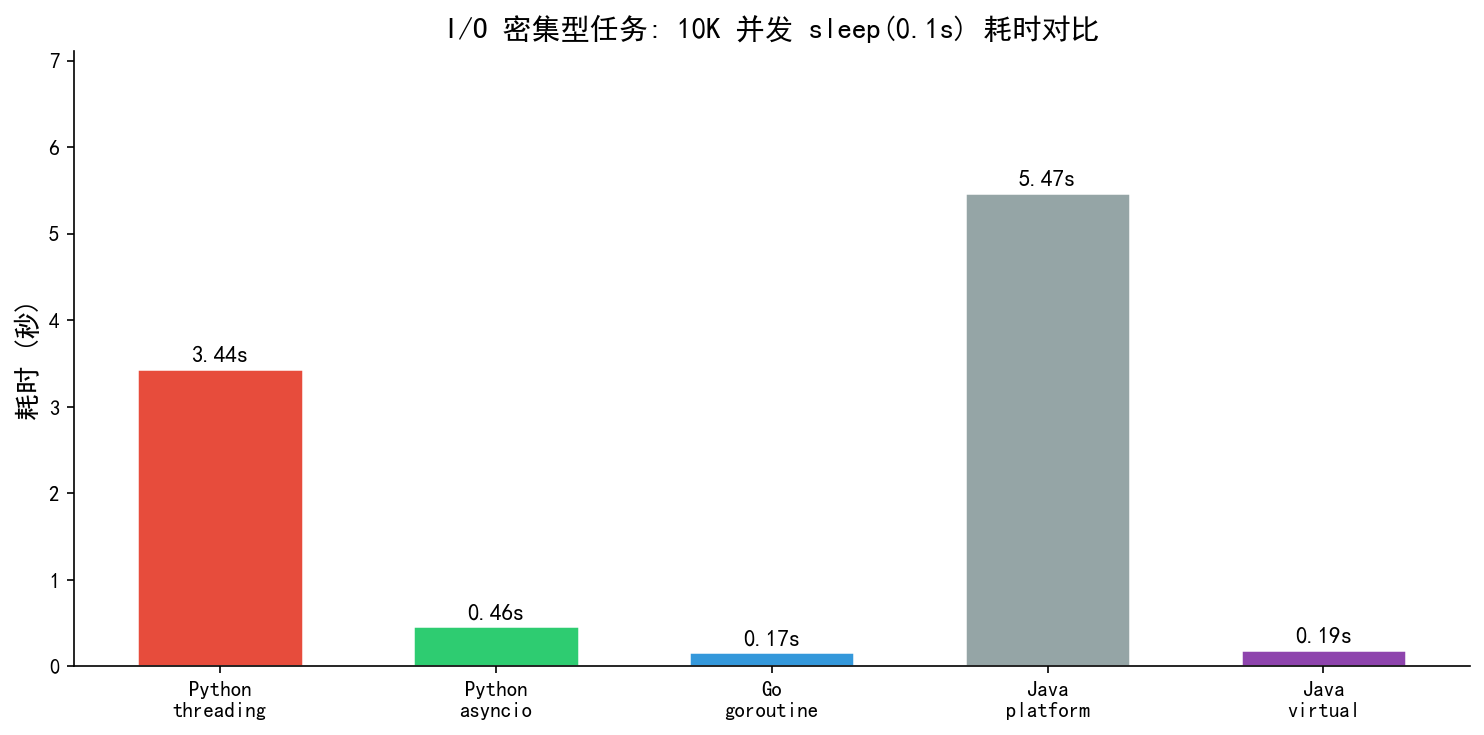
\includegraphics[width=0.72\textwidth]{fig/io_throughput.png}

  \vspace{0.1cm}
  {\footnotesize \textbf{读图方式：}协程/虚拟线程不是让 sleep 更短，而是让 10000 个等待任务不占用 10000 个内核线程。}
\end{frame}

\begin{frame}{实验结果：CPU 密集型与上下文切换}
  \begin{columns}[T]
    \begin{column}{0.48\textwidth}
      \textbf{CPU 密集型 (fib(25) x1000)}\\[0.2cm]
      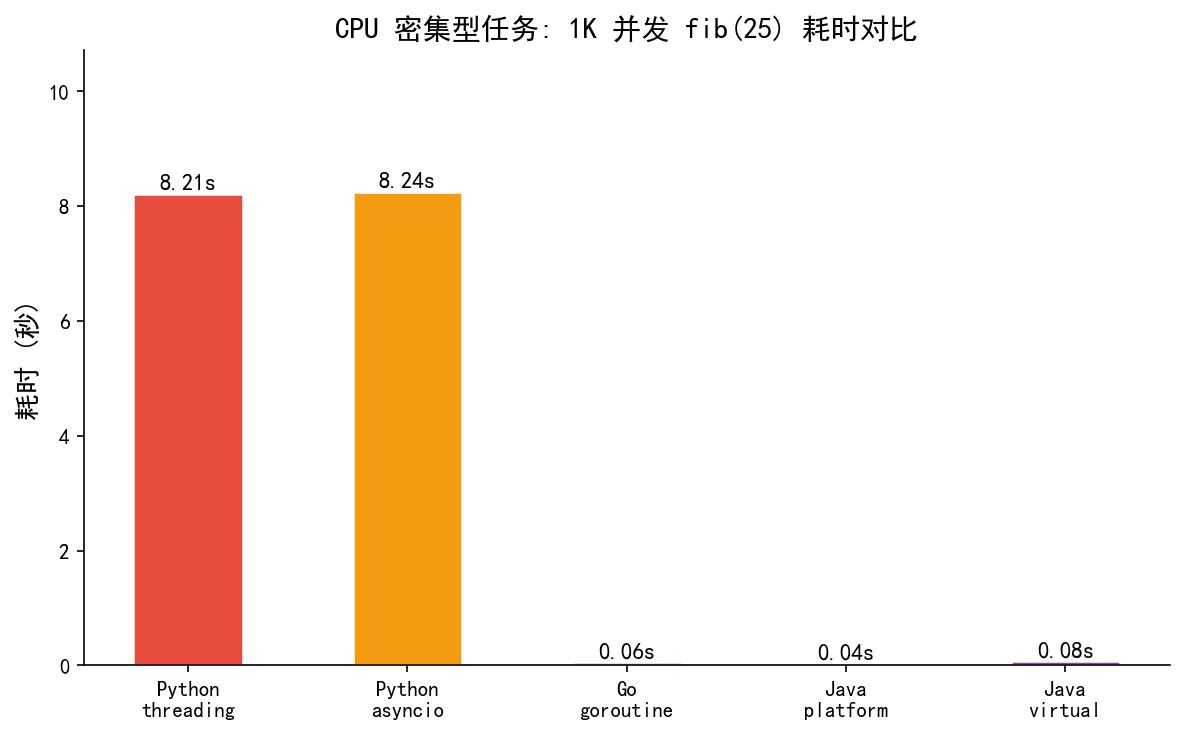
\includegraphics[width=\textwidth]{fig/cpu_benchmark.png}

      \vspace{0.1cm}
      {\tiny 结论：CPU 密集时协程本身无优势，多核调度/线程池才是关键}
    \end{column}
    \begin{column}{0.48\textwidth}
      \textbf{上下文切换开销 (ns/次)}\\[0.2cm]
      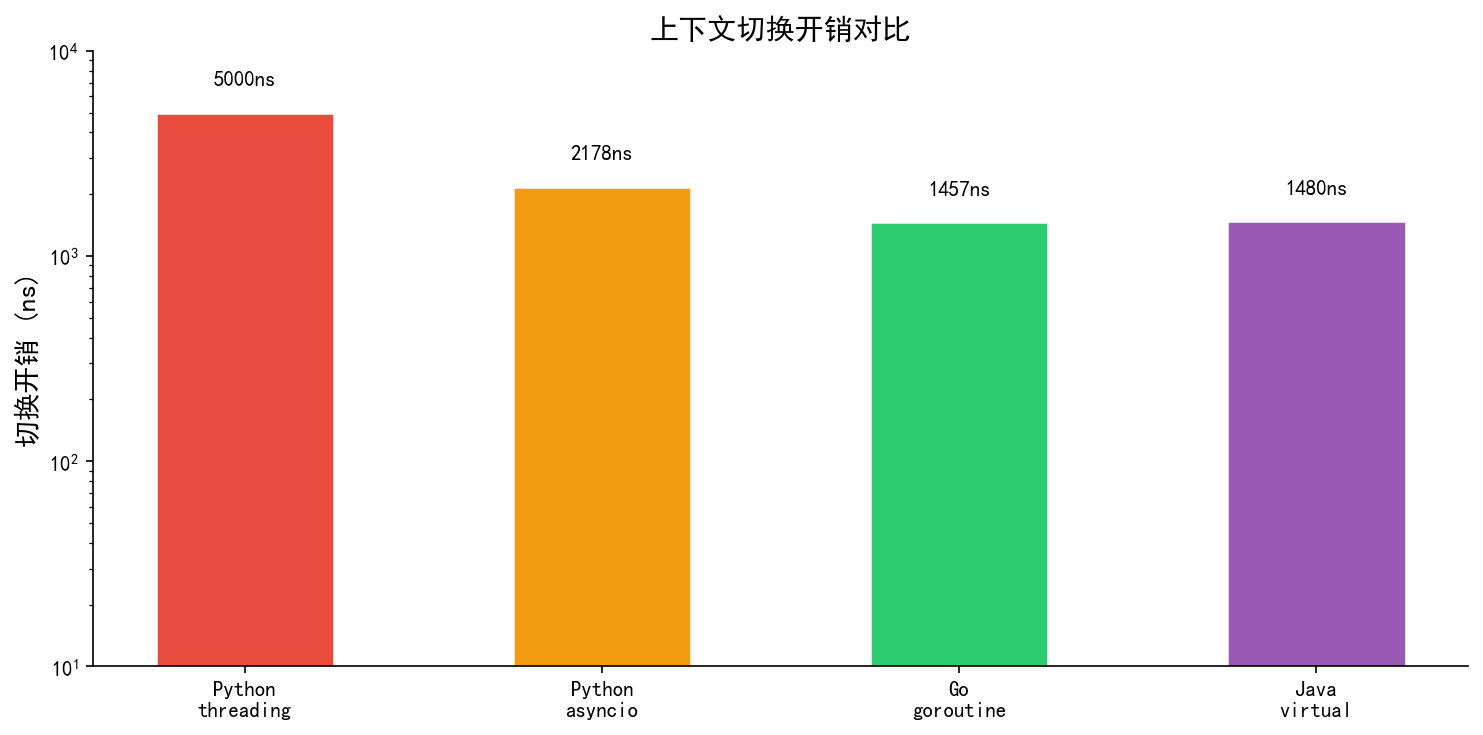
\includegraphics[width=\textwidth]{fig/switch_overhead.png}

      \vspace{0.1cm}
      {\tiny 注：各语言微基准语义不完全等价，只比较量级}
    \end{column}
  \end{columns}
\end{frame}

\begin{frame}{实验洞察与易踩的坑}
  \small
  \begin{columns}[T]
    \begin{column}{0.48\textwidth}
      \begin{exampleblock}{关键发现}
        \begin{itemize}
          \item \textbf{I/O 密集}：协程/虚拟线程优势显著
          \item \textbf{高并发等待}：少量内核线程承载大量逻辑任务
          \item \textbf{CPU 密集}：协程本身\textbf{不会加速计算}
        \end{itemize}
      \end{exampleblock}
    \end{column}
    \begin{column}{0.48\textwidth}
      \textbf{三个陷阱}\\[0.1cm]
      \begin{alertblock}{陷阱 1：阻塞调用毒化}
        在 async 里调用同步 I/O，会卡住事件循环或 carrier。
      \end{alertblock}
      \begin{alertblock}{陷阱 2：未结构化并发}
        协程泄漏会变成资源泄漏；优先使用 TaskGroup/errgroup。
      \end{alertblock}
      \begin{alertblock}{陷阱 3：误用做 CPU 加速}
        协程只省等待和切换；CPU 瓶颈请上多核/SIMD/GPU。
      \end{alertblock}
    \end{column}
  \end{columns}
\end{frame}

\begin{frame}{实验口径与局限}
  \small
  \begin{itemize}
    \item \textbf{I/O 测试}：10000 个 sleep(0.1s) 任务，模拟大量请求等待；它衡量的是调度和等待管理，不是网络协议栈真实性能。
    \item \textbf{CPU 测试}：fib(25) 用来展示 ``协程不自动加速计算''；Go/Java 的优势来自多核调度，不来自协程语义本身。
    \item \textbf{切换测试}：Python asyncio、Go channel、Java sleep(0) 的操作不完全同构，适合看数量级，不适合做精确排名。
    \item \textbf{内存测试}：Python RSS 为脚本记录值，跨语言峰值 RSS 未统一采样；最终结论以耗时和机制解释为主。
  \end{itemize}
\end{frame}

% ================================================================
%  第八部分：选型与总结
% ================================================================
\section{选型建议与总结}

\begin{frame}{选型决策树}
  \begin{center}
  \begin{tikzpicture}[
    node distance=0.5cm,
    decision/.style={diamond, draw=blue!60, fill=blue!5, minimum width=2cm, minimum height=0.8cm, align=center, font=\scriptsize, inner sep=1pt},
    result/.style={rectangle, rounded corners, draw=green!60, fill=green!5, minimum width=1.5cm, minimum height=0.6cm, align=center, font=\scriptsize},
    arr/.style={-{Stealth[length=2mm]}, thick},
  ]
    \node[decision] (start) {瓶颈在？};
    \node[result, below left=0.6cm and 1cm of start] (cpu) {多线程/多进程/GPU};
    \node[decision, below right=0.6cm and 1cm of start] (io) {并发量？};
    \draw[arr] (start) -- node[above left, font=\tiny] {CPU} (cpu);
    \draw[arr] (start) -- node[above right, font=\tiny] {I/O} (io);

    \node[result, below left=0.6cm and 0.3cm of io] (small) {OS 线程足够};
    \node[decision, below right=0.6cm and 0.3cm of io] (big) {语言生态？};
    \draw[arr] (io) -- node[above left, font=\tiny] {$<$1k} (small);
    \draw[arr] (io) -- node[above right, font=\tiny] {1k--百万} (big);

    \node[result, below left=0.5cm and 0.8cm of big] (go) {Go: goroutine};
    \node[result, below left=0.5cm and 0cm of big] (java) {Java 21 虚拟线程};
    \node[result, below right=0.5cm and 0cm of big] (py) {asyncio+uvloop};
    \node[result, below right=0.5cm and 0.8cm of big] (cpp) {C++20/Rust async};
    \draw[arr] (big) -- (go);
    \draw[arr] (big) -- (java);
    \draw[arr] (big) -- (py);
    \draw[arr] (big) -- (cpp);
  \end{tikzpicture}
  \end{center}

  \vspace{0.2cm}
  \centering
  \small
  想\textbf{最少改代码} → Java 21 虚拟线程 / Go \quad
  想\textbf{最快上手} → Python asyncio + FastAPI \quad
  想\textbf{极致性能} → Rust + tokio / C++20 + io\_uring
\end{frame}

\begin{frame}{总结}
  \begin{block}{协程到底带来了什么？}
    \begin{itemize}
      \item \textbf{思想}：把\textit{手写的事件循环}交给\textit{编译器 + 运行时}
      \item \textbf{技术栈}：编译器（状态机）+ 运行时（调度器 + IO poller）+ OS（epoll/io\_uring）
      \item \textbf{效果}：用线性代码扛百万并发 I/O
    \end{itemize}
  \end{block}

  \begin{exampleblock}{趋势}
    Java 21 虚拟线程 + Rust 异步生态 + io\_uring，三者会把协程进一步「无感化」。
  \end{exampleblock}

  \begin{center}
    \large
    \textbf{协程不是新东西}（1958 年 Conway 就提了），\\
    但它在 2010s--2020s 复兴，是因为：\\
    \textcolor{blue!70}{\textbf{云时代的并发量级 × 多核硬件 × 编译器技术成熟}}，三者同时到位。
  \end{center}
\end{frame}

% ================================================================
%  AI 使用说明
% ================================================================
\section{AI 使用说明}

\begin{frame}{AI 使用说明}
  \begin{enumerate}
    \item \textbf{信息搜集}：用 ChatGPT / Notion AI 检索 C++20 协程标准、Go GMP 调度器、Java 21 JEP-444、C\# 状态机生成等技术细节，作为一手资料的「索引」。
    \item \textbf{结构梳理}：用 AI 列出「演进—原理—语言—实验—总结」骨架，再人工调整顺序和侧重。
    \item \textbf{图示生成}：TikZ 图由本人手写并让 AI 校正语法（\textbf{非截图}）。
    \item \textbf{实验代码}：AI 给出基准代码雏形 → 我在本机运行、修正、补齐计时与内存采集 → 真实数据替换参考量级。
    \item \textbf{文字润色}：所有幻灯片中文字均由本人撰写，AI 仅做术语校对和长句拆分。
    \item \textbf{核查}：对每条「数字 / 版本号 / 论断」均回查官方文档/JEP/PEP，避免幻觉。
  \end{enumerate}
\end{frame}

% ================================================================
%  参考资料
% ================================================================
\section{参考资料}

\begin{frame}{参考资料}
  \small
  \textbf{标准 / 提案}
  \begin{itemize}
    \item ISO C++20: {[}dcl.fct.def.coroutine{]}
    \item JEP 444: Virtual Threads (Java 21)
    \item PEP 492 / 525 / 530: Python coroutines \& async generators
  \end{itemize}

  \textbf{经典文献}
  \begin{itemize}
    \item Conway M. \textit{Design of a Separable Transition-Diagram Compiler}, 1963
    \item Moura \& Ierusalimschy \textit{Revisiting Coroutines}, TOPLAS 2009
  \end{itemize}

  \textbf{运行时实现}
  \begin{itemize}
    \item Go runtime source: runtime/proc.go (GMP)
    \item OpenJDK Loom 项目 wiki
    \item libuv / tokio / asio 设计文档
  \end{itemize}

  \textbf{必读博文}
  \begin{itemize}
    \item \textit{What Color is Your Function} — Bob Nystrom
    \item \textit{Why goroutines are not lightweight threads} — Dave Cheney
  \end{itemize}
\end{frame}

% ================================================================
%  Q&A
% ================================================================
\begin{frame}
  \begin{center}
    \vspace{2cm}
    {\Huge\textbf{Q\&A}}\\[1cm]
    {\Large 欢迎提问 · 谢谢聆听}\\[1cm]
    {\normalsize 演示文件 + 实验代码}
  \end{center}
\end{frame}

\end{document}
